% !TeX TXS-program:compile = txs:///lualatex/[--shell-escape]
\documentclass[a4paper,14pt,russian]{extreport}

\usepackage[english,main=russian]{babel}

%\usepackage{newtxmath}
\usepackage[no-math]{fontspec}
\usepackage{polyglossia}

\defaultfontfeatures{Ligatures = TeX, Mapping = tex-text}

\setmainlanguage[babelshorthands = true]{russian}
\setotherlanguage{english}

\setmainfont{Times New Roman}

\newfontfamily\cyrillicfont{Times New Roman}
\newfontfamily\englishfont{Times New Roman}

\usepackage[
	left=30mm,
	right=10mm, 
	top=20mm,
	bottom=20mm,
]{geometry}

\makeatletter
	\renewcommand\LARGE{\@setfontsize\LARGE{22pt}{20}}
	\renewcommand\Large{\@setfontsize\Large{20pt}{20}}
	\renewcommand\large{\@setfontsize\large{16pt}{20}}
\makeatother

\usepackage{microtype} % Настройка переносов
\sloppy
\usepackage{nicematrix}
\usepackage{setspace} % Настройка межстрочного интервала
\onehalfspacing

\usepackage{indentfirst} % Настройка абзацного отступа
\setlength{\parindent}{12.6mm}

\usepackage[unicode,hidelinks]{hyperref}
\usepackage{xifthen}

\usepackage{colortbl}

\usepackage[normalem]{ulem}
% Текст под линией 
\newcommand*{\undertext}[2]{%
	\begin{tabular}[t]{@{}c@{}}%
		#1\\\relax\scriptsize(#2)%
	\end{tabular}
}

% горизонтальная линия
\makeatletter
\newcommand{\vhrulefill}[1]
{
	\leavevmode\leaders\hrule\@height#1\hfill \kern\z@
}

\usepackage[figure,table]{totalcount} % Подсчет изображений, таблиц
\usepackage{rotating} % Поворот изображения вместе с названием
\usepackage{lastpage} % Для подсчета числа страниц

\usepackage{titlesec}
\usepackage{titletoc}
\usepackage{tocloft}

\setcounter{tocdepth}{5}

\setlength{\cftbeforetoctitleskip}{-25pt}
\renewcommand{\cfttoctitlefont}{\large\bfseries}

\renewcommand{\cftchapfont}{\large\bfseries}
\renewcommand{\cftsecfont}{\large}
\renewcommand{\cftchapleader}{\cftdotfill{\cftdotsep}}

\setlength{\cftbeforepartskip}{10pt}


\setcounter{secnumdepth}{5}

\titleformat{\part}[block]
{\large\bfseries}{\thechapter}{0.5em}{\large\centering}

\titleformat{\chapter}[block]
% {\large\bfseries}{\thechapter}{0.5em}{\large\raggedright}
{\hspace{\parindent}\large\bfseries}{\thechapter}{0.5em}{\large\raggedright}

\titleformat{\section}[block]
% {\large\bfseries}{\thesection}{0.5em}{\large\raggedright}
{\hspace{\parindent}\large\bfseries}{\thesection}{0.5em}{\large\raggedright}
\renewcommand{\thesection}{\arabic{chapter}.\arabic{section}.}

\titleformat{\subsection}[block]
{\hspace{\parindent}\large\bfseries}{\thesubsection}{0.5em}{\large\raggedright}
\renewcommand{\thesubsection}{\arabic{chapter}.\arabic{section}.\arabic{subsection}.}

\titleformat{\subsubsection}[block]
{\hspace{\parindent}\large\bfseries}{\thesubsubsection}{0.5em}{\large\raggedright}
\renewcommand{\thesubsubsection}{\arabic{chapter}.\arabic{section}.\arabic{subsection}.\arabic{subsubsection}.}

\titleclass{\part}{top}
\titlespacing*{\part}{12.5mm}{-22pt}{10pt}

\titlespacing{\chapter}{12.5mm}{-22pt}{10pt}
\titlespacing{\section}{12.5mm}{10pt}{10pt}
\titlespacing{\subsection}{12.5mm}{10pt}{10pt}
\titlespacing{\subsubsection}{12.5mm}{10pt}{10pt}

% ---------------------------------------- CAPTION --------------------------------- %

\usepackage[
	labelsep=endash,
	singlelinecheck=false,
]{caption}

\captionsetup[figure]{justification=centering}
\captionsetup[table]{justification=raggedleft}
\captionsetup[listing]{justification=raggedright}
\usepackage{caption} %заголовки плавающих объектов

\captionsetup[figure]{name=Рисунок}


% ---------------------------------------- ABBRS --------------------------------- %

\usepackage{enumitem}
\newcounter{descriptcount}
\newlist{enumdescript}{description}{2}
\setlist[enumdescript,1]{%
	before={\setcounter{descriptcount}{0}%
		\renewcommand*\thedescriptcount{\arabic{descriptcount})}}
	,font=\stepcounter{descriptcount}\thedescriptcount~
}
\setlist[enumdescript,2]{%
	before={\setcounter{descriptcount}{0}%
		\renewcommand*\thedescriptcount{\roman{descriptcount}}}
	,font=\stepcounter{descriptcount}\thedescriptcount~
}

\def\labelitemi{--} % Изменение буллета для списков


% ---------------------------------------- TABLE  ----------------------------------------

\usepackage{xcolor}
\usepackage{tabularx}
\usepackage{booktabs}
\usepackage{multirow}

\newcolumntype{O}{>{\centering\arraybackslash}p{0.08\textwidth}}
\newcolumntype{T}{>{\centering\arraybackslash}p{0.3\textwidth}}
\newcolumntype{L}{>{\centering\arraybackslash}p{0.45\textwidth}}
\newcolumntype{P}{>{\centering\arraybackslash}p{0.2\textwidth}}
\newcolumntype{R}{>{\centering\arraybackslash}p{0.22\textwidth}}
\newcolumntype{F}{>{\centering\arraybackslash}p{0.25\textwidth}}
\newcolumntype{S}{>{\centering\arraybackslash}p{0.15\textwidth}}
\newcolumntype{U}{>{\centering\arraybackslash}p{0.16\textwidth}}
\newcolumntype{N}{>{\centering\arraybackslash}p{0.19\textwidth}}
\newcolumntype{H}{>{\centering\arraybackslash}p{0.13\textwidth}}
\newcolumntype{E}{>{\centering\arraybackslash}p{0.18\textwidth}}
\newcolumntype{G}{>{\centering\arraybackslash}p{0.6\textwidth}}
\newcolumntype{Q}{>{\centering\arraybackslash}p{0.1\textwidth}}
\newcolumntype{C}[1]{>{\centering\arraybackslash}m{#1}}
\usepackage{slashbox}
% ---------------------------------------- FIGURE ----------------------------------------

\usepackage{graphicx}
\usepackage{float}
\usepackage{wrapfig}
\usepackage{tikzscale}
\usepackage[notransparent]{svg}
\svgpath{{assets/}}
\makeatletter
	\let\quote@name\unquote@name
\makeatother


\usepackage{pgfplots}
\pgfplotsset{compat=newest}

% ----------------------------------------- MATH -----------------------------------------

\usepackage{lscape}
\usepackage{afterpage}

\usepackage{amsmath}

\DeclareMathOperator*{\argmax}{arg\,max}
\DeclareMathOperator*{\argmin}{arg\,min}
% ----------------------------------------- LST -----------------------------------------
\usepackage{listings}
\usepackage{courier}

%\usepackage[cache=false, newfloat]{minted}
%\newenvironment{code}{\captionsetup{type=listing}}{}
\renewcommand{\lstlistingname}{Листинг}

\newcommand{\codefont}{\fontfamily{pcr}}
\newcommand{\keywordsfont}{\fontfamily{pcr}\bfseries}

%\usepackage{listings-golang} % import this package after listings
%\usepackage{minted}
% \lstset{
% 	basicstyle=\codefont\footnotesize,
% 	keywordstyle=\keywordsfont\color{black},
% 	numbers=left,
% 	numberstyle=\fontfamily{pcr}\tiny,
% 	showstringspaces=false,
% 	numbersep=10pt,
% 	tabsize=4,
% 	frame=tblr,	
% 	xleftmargin=25pt,
% 	framexleftmargin=18pt,
% 	framexrightmargin=-5pt,
% %	framexbottommargin=10pt,
% %	linewidth=0.95\pagewidth
% }

\usepackage[ruled,linesnumbered,resetcount,algochapter]{algorithm2e}
\SetKwInput{KwData}{Исходные параметры}
\SetKwInput{KwResult}{Результат}
\SetKwInput{KwIn}{Входные данные}
\SetKwInput{KwOut}{Выходные данные}
\SetKwIF{If}{ElseIf}{Else}{если}{тогда}{иначе если}{иначе}{конец условия}
\SetKwFor{While}{до тех пор, пока}{выполнять}{конец цикла}
\SetKw{KwTo}{от}
\SetKw{KwRet}{возвратить}
\SetKw{Return}{возвратить}
\SetKwBlock{Begin}{начало блока}{конец блока}
\SetKwSwitch{Switch}{Case}{Other}{Проверить значение}{и выполнить}{вариант}{в противном случае}{конец варианта}{конец проверки значений}
\SetKwFor{For}{цикл}{выполнять}{конец$\;$цикла} % очевидный и невероятный костыль
\SetKwFor{ForEach}{для каждого}{выполнять}{конец цикла}
\SetKwRepeat{Repeat}{повторять}{до тех пор, пока}
\SetAlgorithmName{Листинг}{алгоритм}{Список алгоритмов}

% ----------------------------------------- BIBLIO ---------------------------------------

\usepackage{totcount}
%\newtotcounter{citenum} %From the package documentation
%\AtEveryBibitem{\stepcounter{citenum}}

\usepackage[
	style=gost-numeric,
	language=auto,
	autolang=other,
	sorting=none,
	movenames=true,
	maxnames=3,
%	minnames=3,
	]{biblatex}
\usepackage{csquotes}

% Modify the @article style
\DeclareFieldFormat[article]{title}{#1} % Preserve the title as is

\newcounter{totalbibentries}
\newcommand*{\listcounted}{}

\makeatletter
\AtDataInput{%
	\xifinlist{\abx@field@entrykey}\listcounted
	{}
	{\stepcounter{totalbibentries}%
		\listxadd\listcounted{\abx@field@entrykey}}%
}
\makeatother


%\providecommand*{\BibDash}{}
\DeclareFieldFormat{extradate}{}

\DeclareFieldFormat[online]{title}{#1 [Электронный ресурс]}

\DeclareFieldFormat{urldate}{(дата обращения:\addspace\thefield{urlday}\adddot \thefield{urlmonth}\adddot\thefield{urlyear})}

\usepackage{longtable}

\DeclareFieldFormat{url}{\bibstring{urlfrom}, URL:\addcolon\space\url{#1}}

\usepackage{url}
\urlstyle{same}

\usepackage{color} % Цвета для гиперссылок и листингов
\definecolor{comment}{rgb}{0,0.5,0}
\definecolor{plain}{rgb}{0.2,0.2,0.2}
\definecolor{string}{rgb}{0.91,0.45,0.32}
\hypersetup{citecolor=blue}
\hypersetup{citecolor=black}
\newfontfamily\lstfont{Times New Roman}
\usepackage{listings}
\lstset{
	basicstyle=\fontsize{12}{12}\linespread{1.0}\lstfont,
	language=python, % Или другой ваш язык -- см. документацию пакета
	commentstyle=\color{comment},
	numbers=left,
	numberstyle=\tiny,
	stepnumber=1,
	numbersep=5pt,
	xleftmargin =.19in,
	tabsize=4,
	extendedchars=\true,
	breaklines=true,
	keywordstyle=\color{black},
	frame=single,
	stringstyle=\lstfont\color{black}\lstfont,
	showspaces=false,
	showtabs=false,
	showstringspaces=false,
	showstringspaces=false,
	inputencoding=utf8x,
	keepspaces=true,
	captionpos=t,
	breakatwhitespace=false,
}
\DeclareCaptionFont{white}{\color{white}}
\captionsetup[lstlisting]{
	singlelinecheck=false,
	justification=centering,
	labelsep=endash,
}

\usepackage{color}
\usepackage[cache=false, newfloat]{minted}
\newenvironment{code}{\captionsetup{type=listing}}{}
\SetupFloatingEnvironment{listing}{name=Листинг}
\usepackage{float}
\usepackage{amsmath}

\usepackage{tocloft}

% Đặt căn lề trái cho các chương trong mục lục
\cftsetindents{chapter}{0cm}{2.5em}

% % Đặt căn lề trái cho các phần trong mục lục
\cftsetindents{part}{1.25cm}{2.5em}

% % Đặt căn lề trái cho các mục con (section) trong mục lục
\cftsetindents{section}{1cm}{2.5em}

% % Đặt căn lề trái cho các mục con con (subsection) trong mục lục
\cftsetindents{subsection}{1.27cm}{2.5em}
\addbibresource{biblio.bib}
\begin{document}
	%\includepdf{title.pdf}
	% \includepdf[pages=-]{calendar.pdf}
    % \the\cftsubsecindent
	\setcounter{page}{3}
	% %\setupsectionstar
\part*{РЕФЕРАТ}
\addcontentsline{toc}{part}{РЕФЕРАТ}
Расчетно-пояснительная записка содержит \pageref{LastPage} с., \totalfigures\ рис.

\textbf{Ключевые слова}: глубокая подделка, дипфейк, Deepfake, сверточные нейронные сети, глубокое обучение.

Объектом исследования является обнаружения глубокой подделки на изображениях.

Предметом исследования является разработка архитектуры сверточной нейронной сети для решения поставленной задачи.

Целью работы являлась разработка метода обнаружения глубокой подделки на изображениях с использованием сверточной нейронной сети.

Для достижения поставленной цели необходимо выполнить следующие задачи:

\begin{itemize}
    \item[---] изложить особенности предлагаемого метода;
    \item[---] описать основные этапы разрабатываемого метода в виде детализированной диаграммы IDEF0 и схем архитектуры разрабатываемой нейронной сети;
    \item[---] спроектировать структуру программного обеспечения для реализации разрабатываемого метода.
\end{itemize}

\pagebreak
	\renewcommand{\contentsname}{\centerline{СОДЕРЖАНИЕ}} % Переименовать table of contents
        \tableofcontents

	\part*{ВВЕДЕНИЕ}
\addcontentsline{toc}{part}{ВВЕДЕНИЕ}
В современном мире, где скорость и удобство имеют первостепенное значение, система бронирования авиабилетов стала неотъемлемой частью путешествий. Появление интернета и развитие технологий позволили перевести процесс бронирования в онлайн-среду, сделав его доступным и удобным для миллионов людей по всему миру. 

С каждым годом количество пассажиров, пользующихся авиаперевозками, увеличивается. Это обусловлено увеличением доступности авиаперелетов, развитием инфраструктуры и увеличением спроса на туризм. Создание современных систем бронирования позволяет удовлетворить возрастающий спрос на авиаперевозки и обеспечить удобство пользователей.

В сфере авиаперевозок увеличивается конкуренция между авиакомпаниями. Создание современной системы бронирования с удобным интерфейсом, широким выбором рейсов и эффективной системой оплаты позволяет привлечь больше клиентов и укрепить конкурентные позиции.

Целью курсовой работы является разработка системы бронирования авиабилетов. Для ее достижения необходимо выполнить следующие задачи:

\begin{itemize}[label = ---]
  \item описать разрабатываемую систему;
  \item сформулировать требования к системе бронирования авиабилетов;
  \item спроектировать архитектуру распределенной системы;
  \item произвести выбор стека технологий для реализации системы;
  \item реализовать распределенную систему для бронирования авиабилитов.
\end{itemize}



	\chapter{Аналитическая часть}

\section{Описание системы}
Разрабатываемый портал должен представлять собой систему для пукупки авиабилетов. 

Если пользователь хочет купить билет, то ему нужно пройти регистрацию, указав следующую информацию: фамилия, имя, номер телефона, адрес электронной почты, пароль. Для неавторизованных пользователей доступен только просмотр общей информации сайта: списка рейсов с указанием даты и времени отлета, аэропортов отправления и прибытия, цены билета.


\section{Функциональные требования к системе с точки зрения пользователя}
Портал должен обеспечивать реализацию следующих функций.

\begin{enumerate}
    \item Система должна обеспечивать регистрацию и авторизацию пользователей с валидацией вводимых данных.
    \item Аутентификация пользователей.
    \item Разделение всех пользователей на 3 роли:
    \begin{itemize}
      \item неавторизованный пользователь (гость);
	    \item авторизированный пользователь (пользователь);
		  \item администратор.
	\end{itemize}

  \item Предоставление возможностей \textbf{гостю, пользователю, администратору} представленных в таблице \ref{tbl:user-func}.
\end{enumerate}

\newpage
\begin{longtable}{|p{0.5cm}|p{15.5cm}|}
	\caption{Функции пользователей}
	\label{tbl:user-func} \\
	\hline
	
	\begin{rotatebox}[origin=r]{90}
		{ \textbf{Гость}}
	\end{rotatebox}
	& 
	1. Просмотр списка рейсов (включая фильтрацию и сортировку по всем полям); \newline
	2. Регистрация в системе; \newline
	3. Авторизация в системе. \\
	\hline
	
	\begin{rotatebox}[origin=r]{90}
		{ \textbf{Пользователь}}
	\end{rotatebox} 
	& 
    1. Авторизация в системе; \newline
	2. Просмотр списка рейсов (включая фильтрацию и сортировку по всем полям); \newline
	4. Получение информации о данных текущего аккаунта; \newline
	5. Просмотр истории покупок билетов; \newline
	6. Получение детальной информации по билету; \newline
	7. Просмотр списка купленных и сданных билетов; \newline
	8. Покупка билета на выбранный рейс; \newline
    9. Возврат билета. \\
	\hline
	
	\begin{rotatebox}[origin=r]{90}
	{ \textbf{Администратор}}
	\end{rotatebox} 
	& 
    1. Функции пользователя; \newline
	2. Просмотр статистики по сайту. \\	
	\hline
\end{longtable}


\section{Входные данные}
Входные параметры системы представлены в таблице \ref{tbl:input}.

\begin{longtable}{|p{4cm}|p{12cm}|}
	\caption{Входные данные}
	\label{tbl:input} \\
	\hline
	
	\textbf{Сущность} & \textbf{Входные данные} \\
	\hline
	\endfirsthead
	
	\hline
	\textbf{Сущность} & \textbf{Входные данные} \\
	\hline
	\endhead
	
	\hline
	\multicolumn{2}{c}{\textit{Продолжение на следующей странице}}
	\endfoot
	\hline
	\endlastfoot
	
	Регистрация пользователя
	&
	1. \textit{фамилия} не более 256 символов; \newline
	2. \textit{имя} не более 256 символов; \newline
	3. \textit{логин} не более 256 символов; \newline
	4. \textit{пароль} не более 128 символов; \newline
	5. \textit{номер телефона} в формате (+7XXXXXXXXXX); \newline
	6. \textit{роль} администратор или пользователь; \newline
	7. \textit{электронная почта} в формате (*@*.*). \\
	\hline

  Аутентификация пользователя
	&
	1. \textit{логин} не более 256 символов; \newline
	2. \textit{пароль} не более 128 символов. \\
	\hline

  Покупка билета
  & 
	1. \textit{номер рейса}; \newline
	2. \textit{цена билета}; \newline
	3. \textit{флаг, отвечающий за списывание или зачисление бонусов}. \\
	\hline

  Возврат билета
  & 
	1. \textit{идентификатор билета}. \\
	\hline

  Получение детальной информации о билете
  & 
	1. \textit{идентификатор билета}. \\
	\hline

  Фильтр и пагинация полетов
  & 
	1. \textit{номер полета} не более 20 символов; \newline
  2. \textit{минимальная цена} не менее 1; \newline
  3. \textit{максимальная цена} не менее 1; \newline
  4. \textit{минимальное время вылета}; \newline
  5. \textit{максимальное время вылета}; \newline
  6. \textit{аэропорт отправления}; \newline
  7. \textit{аэропорт прибытия}; \newline
	8. \textit{номер страницы} не менее 1; \newline
  9. \textit{размер страницы} не менее 1; \newline
	10. \textit{объектов на странице} не менее 1. \\
	\hline
\end{longtable}
\clearpage

\section{Выходные параметры}
Выходными параметрами системы являются web-страницы. В зависимости от запроса и текущей роли пользователя они содержат следующую информацию (таблица \ref{tbl:output-data}).

\begin{longtable}{|p{0.5cm}|p{15.5cm}|}
	\caption{Выходные параметры}
	\label{tbl:output-data} \\
	\hline
	
	\begin{rotatebox}[origin=r]{90}
		{\textbf{Гость}}
	\end{rotatebox} 
	& 
	1. Список рейсов: \newline
    • \textit{номер полета}; \newline
    • \textit{аэропорт отправления}; \newline
    • \textit{аэропорт прибытия}; \newline
    • \textit{дата и время отлета}; \newline
    • \textit{цена билета}. \\
	\cline{2-2}
    &
  2. Окно авторизации. \\
	\cline{2-2}
    &
	3. Окно регистрации. \\
	\hline
	
	\begin{rotatebox}[origin=r]{90}
		{\textbf{Пользователь}}
	\end{rotatebox} 
	& 
	1. Список рейсов: \newline
    • \textit{номер полета}; \newline
    • \textit{аэропорт отправления}; \newline
    • \textit{аэропорт прибытия}; \newline
    • \textit{дата и время отлета}; \newline
    • \textit{цена билета}. \\
	\cline{2-2}
    &
  2. Список купленных и сданных билетов: \newline
    • \textit{количество бонусов на счету данного пользователя}; \newline
    • \textit{номер полета}; \newline
    • \textit{аэропорт отправления}; \newline
    • \textit{аэропорт прибытия}; \newline
    • \textit{дата и время отлета}; \newline
    • \textit{итоговая цена билета с учетом бонусов}; \newline
    • \textit{статус билета (куплен или сдан)}. \\
	\cline{2-2}
    &
  3. Детальная информация о пользователе, вошедшем в систему; \newline
    • \textit{фамилия}; \newline
    • \textit{имя}; \newline
    • \textit{логин}; \newline
    • \textit{роль}; \newline
    • \textit{электронная почта}; \newline
    • \textit{номер телефона}; \newline
    • \textit{количество бонусов на счету данного пользователя}.\\
	\cline{2-2}
	&
	4. История покупок билетов: \newline
    • \textit{дата и время покупки/сдачи билета}; \newline
    • \textit{количество} начисленных/списанных бонусов. \\
    
  \hline
	\begin{rotatebox}[origin=r]{90}
		{\textbf{Администратор}}
	\end{rotatebox} 
	& 
	1. Список рейсов: \newline
    • \textit{номер полета}; \newline
    • \textit{аэропорт отправления}; \newline
    • \textit{аэропорт прибытия}; \newline
    • \textit{дата и время отлета}; \newline
    • \textit{цена билета}. \\
	\cline{2-2}
    &
  2. Список купленных и сданных билетов: \newline
    • \textit{количество бонусов на счету данного пользователя}; \newline
    • \textit{номер полета}; \newline
    • \textit{аэропорт отправления}; \newline
    • \textit{аэропорт прибытия}; \newline
    • \textit{дата и время отлета}; \newline
    • \textit{итоговая цена билета с учетом бонусов}; \newline
    • \textit{статус билета (куплен или сдан)}. \\
	\cline{2-2}
    &
  3. Детальная информация о пользователе, вошедшем в систему; \newline
    • \textit{фамилия}; \newline
    • \textit{имя}; \newline
    • \textit{логин}; \newline
    • \textit{роль}; \newline
    • \textit{электронная почта}; \newline
    • \textit{номер телефона}; \newline
    • \textit{количество бонусов на счету данного пользователя}.\\
	\cline{2-2}
	&
	4. История покупок билетов: \newline
    • \textit{дата и время покупки/сдачи билета}; \newline
    • \textit{количество начисленных/списанных бонусов}. \\
	\cline{2-2}
  &
  5. Статистика по порталу, собранная через сервис статистики: \newline
    • \textit{метод запроса}; \newline
    • \textit{url запроса}; \newline
    • \textit{числовой статус выполнения запроса}; \newline
    • \textit{время выполнения запроса}. \\
	\hline
\end{longtable}


\section{Состав системы}

Система будет состоять из фронтенда и 9 подсистем:
\begin{itemize}
	\item сервис-координатор;
	\item сервис регистрации и авторизации;
  \item сервис полетов;
  \item сервис билетов;
  \item сервис бонусов;
  \item сервис статистики;
  \item сервис kafka;
  \item сервис consumer;
  \item сервис zookeeper.
\end{itemize}


\subsection{Фронтенд}

\textit{Фронтенд} -- принимает запросы от пользователя по протоколу HTTP и возвращает ответ в виде HTML страниц, файлов стилей и TypeScript.


\subsection{Сервис-координатор}

\textbf{Сервис-координатор} -- сервис, который отвечает за координацию запросов внутри системы. Все сервисы портала (кроме сервиса регистрации и авторизации) должны взаимодействовать друг с другом через сервис-координатор, запросы с фронтенда в том числе сначала должны приходить на сервис-координатор, а затем перенаправляться на нужный сервис. При этом сервис-координатор отвечает за следующие действия.
\begin{enumerate}
	\item получения списка рейсов с пагинацией, фильтрацией и сортировкой от сервиса полетов;
	\item получения аэропортов с фильтрацией от сервиса полетов;
	\item получения списка билетов разных пользователей из сервиса билетов;
	\item получения списка истории покупок билетов пользователя из сервиса бонусов;
	\item получения информации о состоянии бонусного счета пользователя из сервиса бонусов;
  \item оформление покупки билета через сервисы полетов и билетов с учетом бонусного счета пользователя из сервиса бонусов;
	\item возврат билета через сервисы полетов и билетов и с изменением данных в сервисе бонусов (списание раннее начисленных бонусов или начисление ранее списанных).
\end{enumerate}


\subsection{Сервис регистрации и авторизации}

\textbf{Сервис регистрации и авторизации} отвечает за следующие действия.
\begin{enumerate}
	\item Регистрацию нового пользователя;
	\item Аутентификацию пользователя;
	\item Авторизацию пользователя;
  \item Получение данных пользователей;
  \item Изменение данных о пользователе;
	\item Удаление пользователя.
\end{enumerate}

Взаимодействие сервиса регистрации и авторизации с остальными сервисами должно осуществляться по протоколу OpenID Connect. Сам сервис представляет из себя Identity Provider. Сервис регистрации и авторизации в своей работе используют базу данных, которая хранит следующую информацию:
\begin{itemize}
    \item Пользователь:
    \begin{itemize}
        \item \textit{уникальный идентификатор};
        \item \textit{логин};
        \item \textit{имя};
        \item \textit{фамилия};
        \item \textit{захешированный пароль};
        \item \textit{номер телефона};
        \item \textit{электронная почта};
        \item \textit{роль}.
    \end{itemize}
\end{itemize}


\subsection{Сервис полетов}

\textbf{Сервис полетов} реализует следующие функции.
\begin{enumerate}
	\item Получение списка всех рейсов с фильтрацией, сортировкой и пагинацией;
	\item Получение информации о конкретном рейсе;
	\item Создание полета;
	\item Удаление полета;
  \item Получение списка всех аэропортов с пагинацией;
	\item Получение информации о конкретном аэропорте;
	\item Создание аэропорта;
	\item Удаление аэропорта.
\end{enumerate}

Сервис использует в своей работе базу данных:
\begin{itemize}
  \item Полет:
  \begin{itemize}
    \item \textit{уникальный идентификатор};
    \item \textit{номер полета};
    \item \textit{цена билета};
    \item \textit{дата и время отправления};
    \item \textit{идентификатор аэропорта отправления};
    \item \textit{идентификатор аэропорта прибытия}.
  \end{itemize}

  \item Аэропорт:
  \begin{itemize}
    \item \textit{уникальный идентификатор};
    \item \textit{название};
    \item \textit{город};
    \item \textit{страна}.
  \end{itemize}
\end{itemize}


\subsection{Сервис билетов}

\textbf{Сервис билетов} реализует следующие функции.
\begin{enumerate}
	\item Получение списка билетов всех пользователей с фильтрацией, сортировкой и пагинацией;
	\item Получение информации о конкретном билете;
	\item Создание билета;
	\item Изменение билета;
	\item Удаление билета.
\end{enumerate}

Сервис использует в своей работе базу данных:
\begin{itemize}
  \item Билет:
  \begin{itemize}
    \item \textit{уникальный идентификатор};
    \item \textit{uuid билета};
    \item \textit{логин пользователя};
    \item \textit{номер полета};
    \item \textit{цена};
    \item \textit{статус} (PAID/CANCELED).
  \end{itemize}
\end{itemize}


\subsection{Сервис бонусов}

\textbf{Сервис бонусов} реализует следующие функции.
\begin{enumerate}
	\item Получение списка бонусных счетов всех пользователей с фильтрацией, сортировкой и пагинацией;
	\item Получение информации о конкретном бонусном счете;
	\item Создание бонусного счета;
	\item Изменение бонусного счета;
	\item Удаление бонусного счета;
	\item Получение списка историй начисления и списания бонусов всех пользователей с фильтрацией и сортировкой;
	\item Получение информации о конкретной истории;
	\item Создание истории;
	\item Изменение истории;
	\item Удаление истории;
\end{enumerate}

Сервис использует в своей работе базу данных:
\begin{itemize}
  \item Бонусный счет:
  \begin{itemize}
    \item \textit{уникальный идентификатор};
    \item \textit{логин пользователя};
    \item \textit{статус клиента} (BRONZE/SILVER/GOLD);
    \item \textit{баланс}.
  \end{itemize}

  \item История изменения бонусного счета:
  \begin{itemize}
    \item \textit{уникальный идентификатор};
    \item \textit{идентификатор бонусного счета};
    \item \textit{время покупки/возврата билета};
    \item \textit{количество списанных/начисленных бонусов};
    \item \textit{тип операции} (бонусы начислены или списаны).
  \end{itemize}
\end{itemize}


\subsection{Сервис статистики}

\textbf{Сервис статистики} -- сервис, который отвечает за запись событий сервиса координатора в базу данных для осуществления возможности быстрого обнаружения, локализации и воспроизведения ошибки в случае её возникновения. Дает возможность получить статистику с пагинацией.

Сервис использует в своей работе базу данных:
\begin{itemize}
  \item Статистика:
  \begin{itemize}
    \item \textit{уникальный идентификатор};
    \item \textit{метод запроса} GET/POST/PATCH/DELETE/OPTIONS;
    \item \textit{url запроса};
    \item \textit{числовой статус выполнения запроса};
    \item \textit{время выполнения запроса}.
  \end{itemize}
\end{itemize}


\subsection{Сервис kafka}

\textbf{Сервис kafka} \cite{kafka} -- сервис, который необходим для сервиса статистики для сбора и обработки данных в реальном времени, что позволяет анализировать пользовательскую активность. Kafka поддерживает высокие объёмы данных и легко масштабируется, обеспечивая надёжную работу даже при значительных нагрузках. Благодаря встроенной отказоустойчивости и гарантии доставки сообщений, система статистики не потеряет важные данные при сбоях.


\subsection{Сервис consumer}

\textbf{Сервис consumer} -- сервис, который нужен kafka для получения, обработки и анализа данных, поступающих от producer в реальном времени. Kafka действует как посредник, обеспечивая доставку сообщений между различными сервисами, что позволяет consumer-серверам асинхронно получать данные и обрабатывать их по мере поступления. Это важно для поддержания высокой производительности и отказоустойчивости, так как Kafka распределяет нагрузку между несколькими consumer-серверами, помогая избежать перегрузки. Также Kafka гарантирует надёжную доставку сообщений, что позволяет consumer корректно обрабатывать каждое сообщение без риска потери данных. Наконец, она обеспечивает возможность параллельной обработки данных, что ускоряет анализ больших объёмов информации.


\subsection{Сервис zookeeper}

\textbf{Сервис zookeeper} \cite{zookeeper} -- сервис, который нужен kafka для управления и координации различных компонентов в своей распределённой системе. Вот ключевые задачи, которые решает Zookeeper в Kafka.

\begin{enumerate}
  \item Координация кластеров: Zookeeper помогает координировать работу брокеров (серверов Kafka) внутри кластера, отслеживая их состояние. Он сообщает Kafka о том, какие узлы доступны и активно работают, обеспечивая бесперебойное взаимодействие между ними.
  \item Управление метаданными: Zookeeper хранит важную информацию о топиках, партициях и распределении лидеров партиций среди брокеров. Это нужно для того, чтобы потребители (consumers) и производители (producers) могли эффективно взаимодействовать с нужными данными в кластере.
  \item Обнаружение лидера: Zookeeper определяет лидера для каждой партиции Kafka, который отвечает за запись и чтение данных. В случае сбоя одного из брокеров Zookeeper автоматически выбирает нового лидера для партиции, чтобы поддерживать непрерывную работу.
  \item Отказоустойчивость: Zookeeper обеспечивает высокую доступность и надёжность кластера Kafka, помогая восстанавливать компоненты после сбоев и поддерживать согласованное состояние всех узлов системы.
  Управление доступом: Zookeeper управляет доступом клиентов к Kafka и координирует изменения конфигурации, обеспечивая стабильность и безопасность работы кластера.
  \item Таким образом, Zookeeper является критически важным компонентом для обеспечения координации, отказоустойчивости и управления Kafka-кластером.
\end{enumerate}


\section{Требования к программной реализации}
\begin{enumerate}
  \item Требуется использовать СОА (сервис-ориентированную архитектуру) для реализации системы.
	\item Система состоит из микросервисов. Каждый микросервис отвечает за свою область логики работы приложения и должны быть запущены изолированно друг от друга.
	\item При необходимости, каждый сервис имеет своё собственное хранилище,  запросы между базами запрещены.
	\item При разработке базы данных необходимо учитывать, что доступ к ней должен осуществляться по протоколу TCP.
  \item Необходимо  реализовать  один  web-интерфейс  для  фронтенда.  Интерфейс  должен  быть  доступен  через  тонкий  клиент (браузер).
  \item Для межсервисного взаимодействия использовать HTTP (придерживаться RESTful).
  \item Выделить Gateway Service как единую точку входа и межсервисной коммуникации. В системе не должно осуществляться горизонтальных запросов.
	\item Необходимо предусмотреть авторизацию пользователей через интерфейс приложения.
	\item Код хранить на Github, для сборки использовать Github Actions.
	\item Каждый сервис должен быть завернут в docker.
\end{enumerate}


\section{Функциональные требования к подсистемам}

\textbf{Фронтенд} -- серверное  приложение, предоставляет пользовательский интерфейс и внешний API системы, при  разработке которого нужно учитывать следующее:
\begin{itemize}
  \item должен  принимать  запросы  по  протоколу  HTTP и формировать ответы пользователям в формате HTML;
	\item в зависимости от типа запроса должен отправлять последовательные запросы в соответствующие микросервисы;
  \item запросы к микросервисам необходимо осуществлять по протоколу HTTP;
  \item данные необходимо передавать в формате JSON;
  \item целесообразно использовать Tailwind для упрощения написания стилей.
\end{itemize}

\textbf{Сервис-координатор} -- это серверное приложение, которое должно отвечать следующим требованиям по разработке:
  \begin{itemize}
    \item обрабатывать запросы в соответствии со своим назначением, описанным в топологии системы;
    \item принимать и возвращать данные в формате JSON по протоколу HTTP;
    \item использовать очередь для отложенной обработки запросов (например, при временном отказе одного из сервисов);
    \item осуществлять деградацию функциональности в случае отказа некритического сервиса (зависит от семантики запроса);
    \item уведомлять сервис статистики о событиях в системе.
  \end{itemize}

 \textbf{Сервис регистрации и авторизации, сервис библиотек, сервис рейтинга, сервис аренды, сервис статистики} -- это серверные приложения, которые должны отвечать следующим требованиям по разработке:
  \begin{itemize}
    \item обрабатывать запросы в соответствии со своим назначением, описанным в топологии системы;
    \item принимать и возвращать данные в формате JSON по протоколу HTTP;
    \item осуществлять доступ к СУБД по протоколу TCP.
  \end{itemize}

\textbf{Сервис kafka, сервис consumer, сервис zookeeper} -- это серверное приложение, которое должно отвечать следующим требованиям по разработке:
  \begin{itemize}
    \item обрабатывать запросы в соответствии со своим назначением, описанным в топологии системы;
    \item принимать и возвращать данные в формате JSON по протоколу HTTP.
  \end{itemize}


\section{Пользовательский интерфейс}
Для реализации пользовательского интерфейса должен быть использован подход MVC (Model-View-Controller). Этот подход к проектированию интерфейса является популярным шаблоном проектирования, который помогает разделить логику приложения на три основных компонента: Модель (Model), Представление (View) и Контроллер (Controller). Этот подход позволяет улучшить структуру приложения, облегчить его тестирование и управление, а также разработка фронтенда и бекенда могут быть полностью разделены между собой, то есть можно вести независимую разработку.

Пользовательский интерфейс в разрабатываемой системе должен обладать следующими характеристиками:
\begin{itemize}
  \item Кроссбраузерность -- способность интерфейса работать практически в любом браузере любой версии. 
  \item <<Плоский» дизайн>> -- дизайн, в основе которого лежит идея отказа от объемных элементов (теней элементов, объемных кнопок и т.д.) и замены их плоскими аналогами.
  \item Расширяемость -- возможность легко расширять и модифицировать пользовательский интерфейс.
\end{itemize}
  
  
\section{Сценарий взаимодействия с приложением}
Приведем пример работы портала на примере выполнения запроса от пользователя на получение списка купленных и сданных билетов.

\begin{enumerate}
  \item На фронтенд приходит запрос пользователя.
  \item Если пользователь был авторизован, то происходит получение токена аторизации. Затем выполняется запрос к сервису-координатору. Если данные корректны (данные поступили в ожидаемом формате) и проверка JWT-токена (проверка того, что токен был подписан известным серверу ключом и того, что срок действия токена ещё не истёк) (если он истёк или оказался некорректным, пользователю возвращается ошибка), то отправляются запросы на сервисы билетов и бонусов. 
  \item Выполняются запросы к соответствующим эндпоинтам сервисов билетов для получения даннных о купленных и сданных билетах пользователя, осуществляется проверка корректности полученных данных (данные поступили в ожидаемом формате) и проверка JWT-токена (проверка того, что токен был подписан известным серверу ключом и того, что срок действия токена ещё не истёк). Если он истёк или оказался некорректным, пользователю возвращается ошибка. При успешной проверке токена сервис возвращает список билетов сервису-координатору, который агрегирует полученные данные с балансом бонусного счета и происходит возврат результата на фронтенд.
  \item Если ошибки нигде не произошло, то производится генерация HTML содержимого страницы ответа пользователю с использованием данных, полученных от сервиса-координатора. В ином случае генерируется страница с описанием ошибки.
\end{enumerate}

	\chapter{Конструкторская часть}

\section{Концептуальный дизайн}
Для создания функциональной модели портала, отражающей его основные функции и потоки информации наиболее наглядно использовать нотацию IDEF0. На рисунке \ref{fig:idef0-0} приведена концептуальная модель системы. На рисунке \ref{fig:idef0-1} представлена детализированная концептуальная модель системы в нотации IDEF0.

\begin{figure}[h!]
	\begin{center}
		{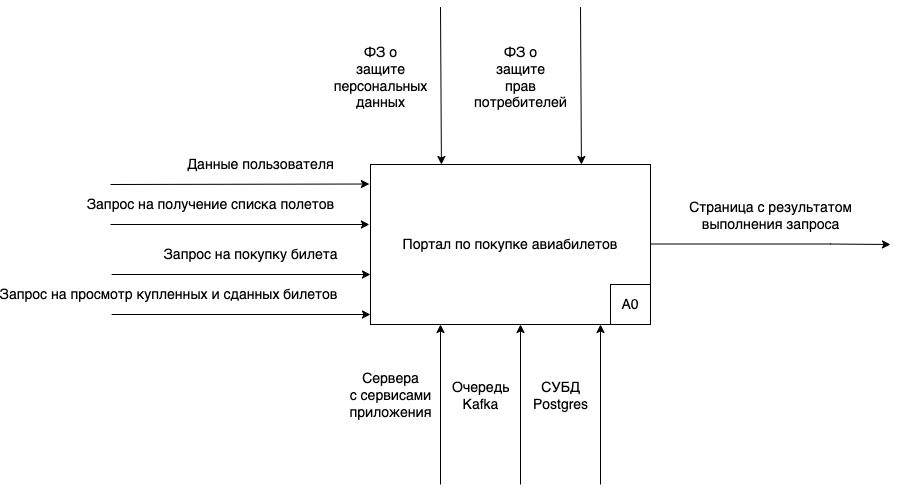
\includegraphics[scale = 0.5, angle=0]{img/idef0/idef0-0.png}}
		\caption{Концептуальная модель системы в нотации IDEF0}
		\label{fig:idef0-0}
	\end{center}
\end{figure}


\begin{figure}[h!]
	\begin{center}
		{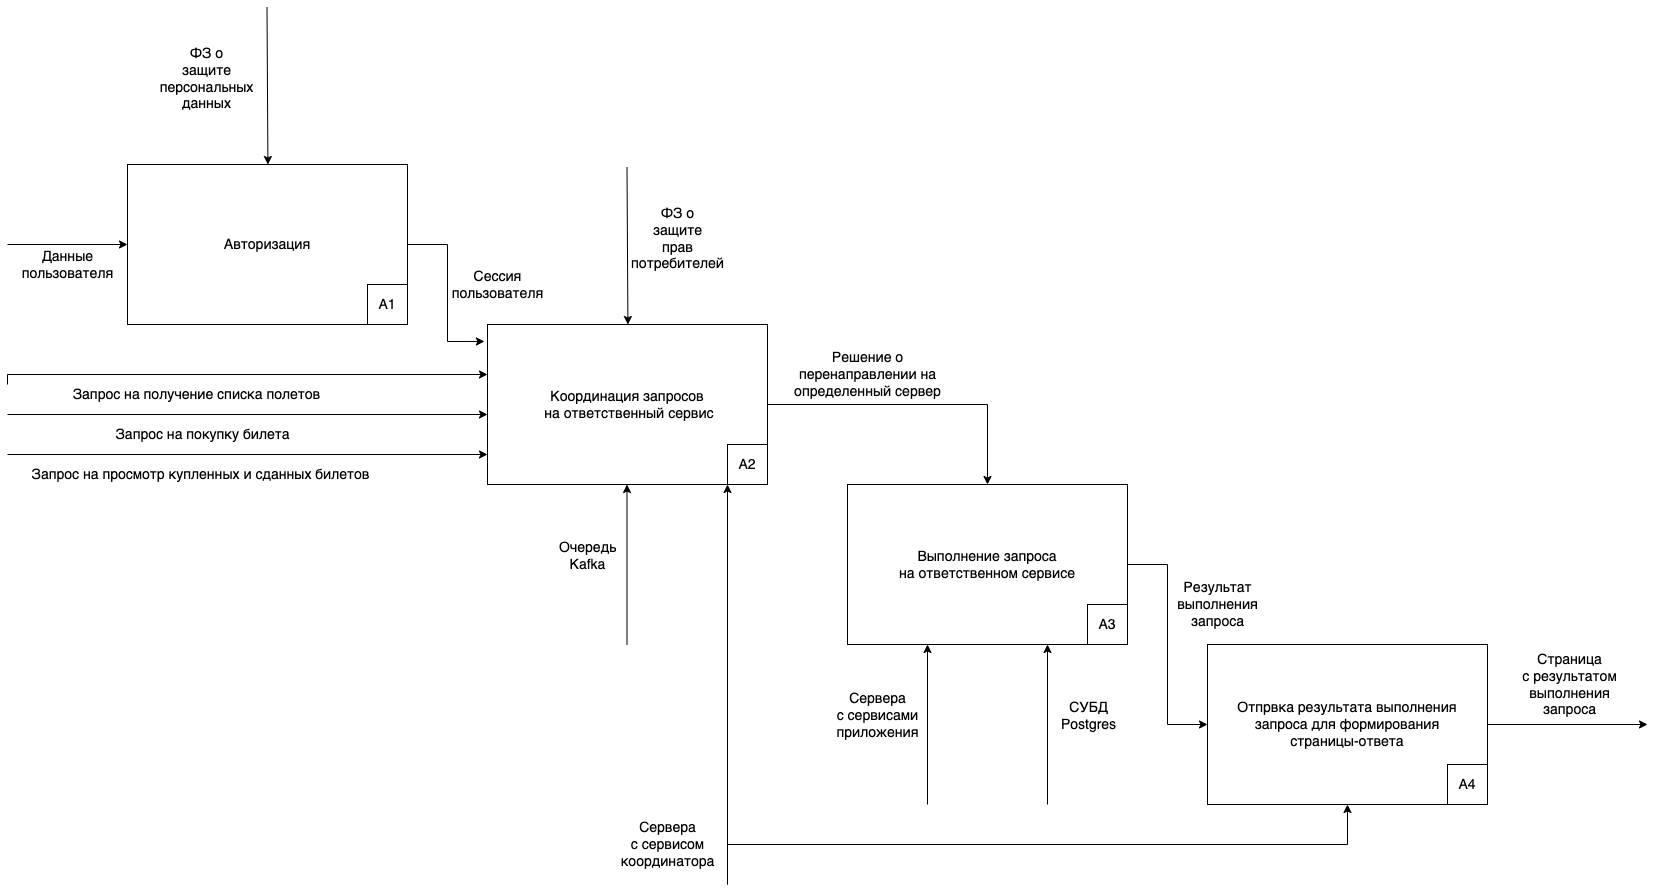
\includegraphics[scale = 0.4, angle=90]{img/idef0/idef0-1.png}}
		\caption{Детализированная концептуальная модель системы в нотации IDEF0}
		\label{fig:idef0-1}
	\end{center}
\end{figure}


\clearpage
\section{Сценарии функционирования системы}

\textbf{Регистрация пользователя}
\begin{enumerate}
	\item Пользователь нажимает на кнопку <<Зарегистрироваться>> в интерфейсе.
	\item Пользователь перенаправляется на страницу, которая содержит поля для заполнения его данных.
	\item Пользователь вводит данные в форму и для завершения регистрации нажимает на кнопку <<Зарегистрироваться>>, тем самым подтверждая верность своих данных, а также согласие на их обработку и хранение.
	\item Если пользователь с введенным для регистрации логином, почтой или номером телефона уже существует, то клиент получает сообщение об ошибке. При успешной регистрации клиент попадает на страниицу со списком полетов.
\end{enumerate}

\textbf{Авторизация клиента}
\begin{enumerate}
	\item Пользователь нажимает на кнопку <<Авторизоваться>> в интерфейсе.
	\item Пользователь перенаправляется на страницу авторизации, которая содержит поля для заполнения логина и пароля.
	\item Пользователь завершает работу с формой авторизации нажатием кнопки <<Войти>>.
	\item При обнаружении ошибки в данных, пользователь получает сообщение об ошибке; при совпадении данных с записью в базе данных аккаунтов пользователь получает доступ к системе и перенаправляется на страниицу со списком полетов.
\end{enumerate}

\textbf{Покупка билета}
\begin{enumerate}
	\item Пользователь на главной странице видит таблицу со списком список полетов. При желании он может отфильтровать и отсортировать их по каждому полю.
	\item Пользователь нажимает на кнопку <<Купить билет>> у выбранного рейса.
  \item Пользователь выбирает, что делать с бонусами (списать или копить) и нажимает кнопку <<Забронировать>>.
  \item В появившемся модальном окно подтверждения с подробной информацией о выбранном рейсе пользователь нажимает на кнопку <<Подтвердить>>.
	\item Пользователь видит модальное окно с информацией об успешности совершенной покупки и нажимает кнопку <<Окей>>.
\end{enumerate}

\textbf{Возврат купленного билета}
\begin{enumerate}
	\item Для просмотра купленных билетов пользователь переходит на страницу <<Билеты>>, нажимая соответсвующую кнопку в выезжающем боковом меню.
	\item Пользователь попадает на страницу, на которой видит все свои купленные и сданные билеты.
	\item У каждого купленного билета есть кнопка <<Сдать билет>>, на которую нажимает пользователь.
	\item В появившемся модальном окно подтверждения с подробной информацией о выбранном билете пользователь нажимает на кнопку <<Подтвердить>>.
  \item Пользователь видит измененный статус билета на <<Билет сдан>> и обновленный баланс бонусного счета.
\end{enumerate}


\section{Диаграммы прецедентов}
В системе выделены 3 роли: Неавторизованный пользователь, Авторизованный пользователь, Администратор. На рисунках \ref{fig:use-case-non-auth}-\ref{fig:use-case-admin} представлены диаграммы прецедентов для каждой из ролей.

\begin{figure}[H]
	\begin{center}
		{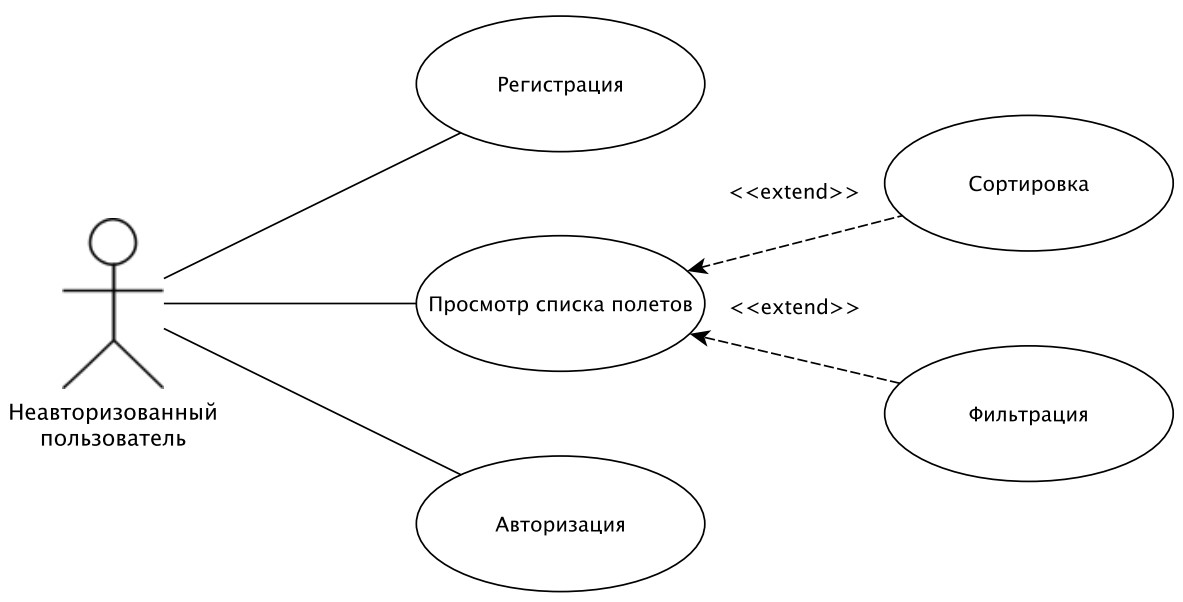
\includegraphics[scale = 0.5]{img/use-case/non-auth-user.jpg}}
		\caption{Диаграмма прецедентов с точки зрения неавторизованного пользователя}
		\label{fig:use-case-non-auth}
	\end{center}
\end{figure}

\begin{figure}[H]
	\begin{center}
		{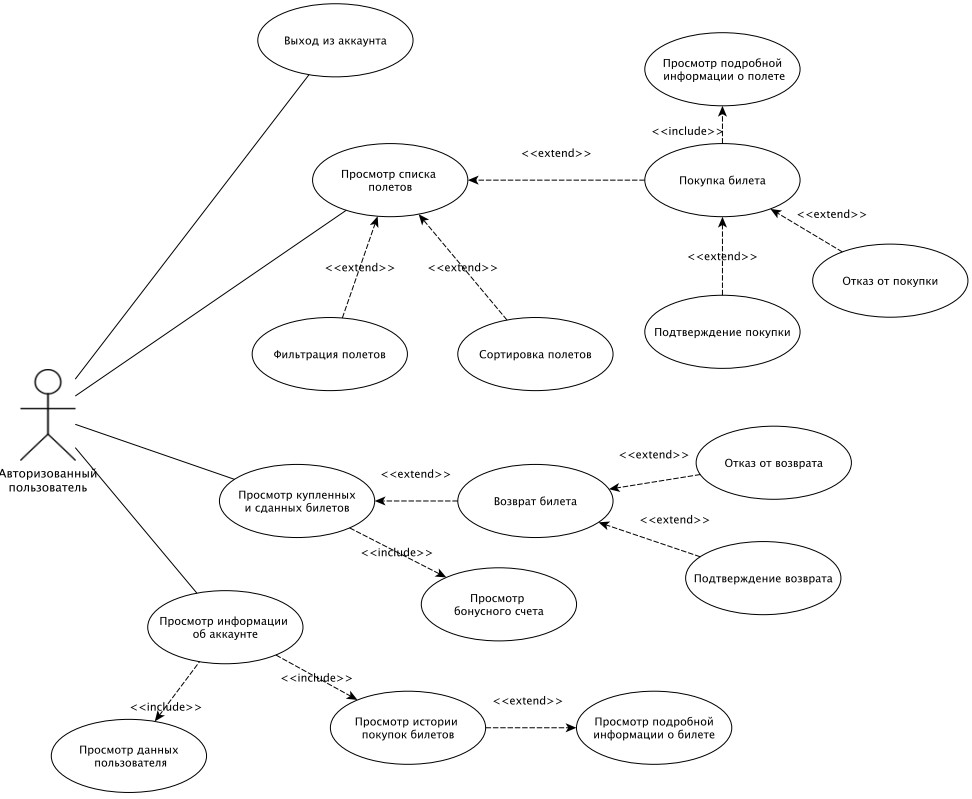
\includegraphics[scale = 0.6]{img/use-case/auth-user.jpg}}
		\caption{Диаграмма прецедентов с точки зрения авторизованного пользователя}
		\label{fig:use-case-auth}
	\end{center}
\end{figure}

\begin{figure}[H]
	\begin{center}
		{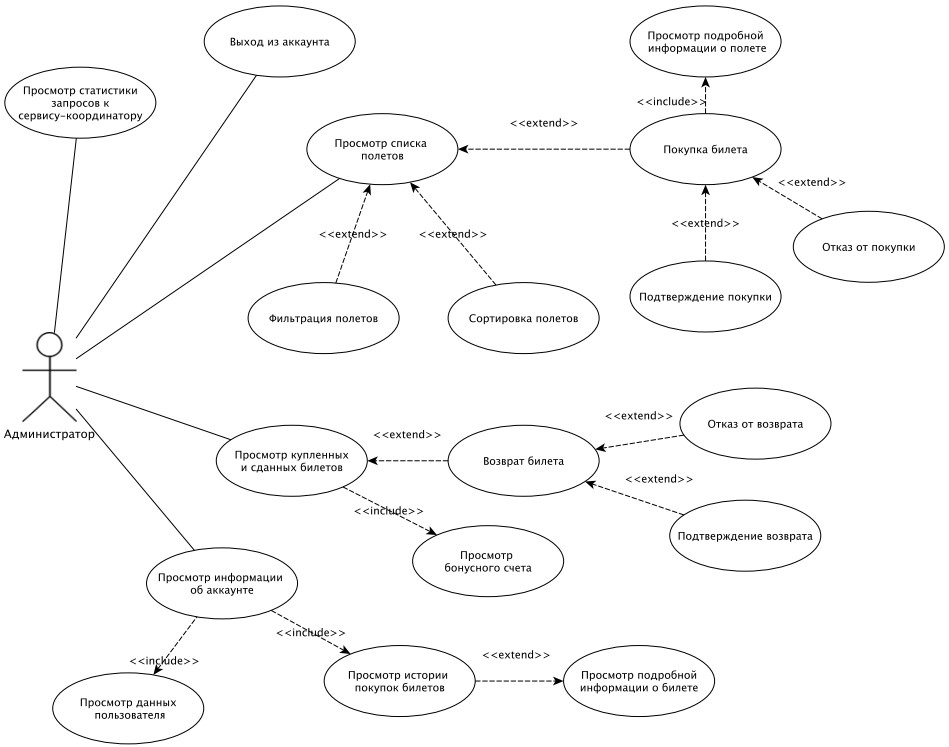
\includegraphics[scale = 0.6]{img/use-case/admin.jpg}}
		\caption{Диаграмма прецедентов с точки зрения администратора}
		\label{fig:use-case-admin}
	\end{center}
\end{figure}

	\chapter{Технологическая часть}

\section{Выбор операционной системы}

Согласно требованиям технического задания, разрабатываемый портал должен обладать высокой доступностью, работать на типичных архитектурах ЭВМ (Intel x86, Intel x64), а так же быть экономически недорогим для сопровождения. Таким образом, требования к ОС следующие.
\begin{itemize}
	\item \textbf{Распространенность}. На рынке труда должно быть много специалистов, способных администрировать распределенную систему, работающую под управлением выбранной операционной системы.
	\item \textbf{Надежность}. Операционная система должна широко использоваться в стабильных проектах, таких как Mail.Ru, Vk.com, Google.com. Эти компании обеспечивают высокую работоспособность своих сервисов, и на их опыт можно положиться.
	\item \textbf{Наличие требуемого программного обеспечения}. Выбор операционной системы не должен ограничивать разработчиков в выборе программного обеспечения, библиотек.
	\item \textbf{Цена}.
\end{itemize}
 
Под данные требования лучше всего подходит ОС Linux, дистрибутив Ubuntu. \textbf{Ubuntu} \cite{ubuntu} — это дистрибутив, использующий ядро Linux. Как и все дистрибутивы Linux, Ubuntu является ОС с открытым исходным кодом, бесплатным для использования. Поставляется как в клиентской (с графическим интерфейсом), так и в серверной (без графического интерфейса) версиями. Ubuntu поставляется с современными версиями ПО. Преимуществом Ubuntu являются низкие требования к квалификации системных администраторов. Однако Ubuntu менее стабильна в работе.


\section{Выбор СУБД}

В качестве СУБД была выбрана \textbf{PostgreSQL} \cite{postgresql}, так как она наилучшим
образом подходит под требования разрабатываемой системы:
\begin{itemize}
	\item Масштабируемость: PostgreSQL поддерживает горизонтальное масштабирование, что позволяет распределить данные и запросы между несколькими узлами базы данных. Это особенно полезно в географически распределенных системах, где данные и пользователи могут быть разбросаны по разным регионам.
	\item Географическая репликация: PostgreSQL предоставляет возможность
настройки репликации данных между различными узлами базы данных, расположенными в разных географических зонах. Это позволяет
обеспечить отказоустойчивость и более быстрый доступ к данным для
пользователей из разных частей нашей страны.
	\item Гибкость и функциональность: PostgreSQL обладает широким набором
функций и возможностей, что делает его подходящим для различных
типов приложений и использования в распределенной среде. Он поддерживает сложные запросы, транзакции, хранимые процедуры и многое
другое.
	\item Надежность и отказоустойчивость: PostgreSQL известен своей надежностью и стабильностью работы. В распределенной географической
системе это особенно важно, поскольку он способен обеспечить сохранность данных и доступность даже при сбоях в отдельных узлах.
\end{itemize}


\section{Выбор языка разработки и фреймворков компонент
портала}

Для разработки бэкенда существует множество языков программирования, каждый из которых имеет свои сильные и слабые стороны, для данного приложения был выбран \textbf{Python} \cite{python} по следующим причинам:

\begin{enumerate}
	\item Простота и скорость разработки: Python позволяет разработчикам писать меньше кода и быстрее реализовывать функциональность, благодаря удобному синтаксису и мощным фреймворкам (Django, Flask, FastAPI). Это особенно важно для стартапов и небольших проектов, где критично быстрое создание прототипов и внедрение изменений.
	\item Широкая экосистема: В Python существует множество готовых библиотек для работы с базами данных, аутентификацией, кэшированием, очередями, обработкой данных и другими задачами бэкенда. Это ускоряет разработку и снижает количество ручной работы.
	\item Поддержка современных технологий: Python активно используется для задач, связанных с машинным обучением, обработкой данных и научными вычислениями. Это делает его выбором номер один для компаний, работающих с большими данными или развивающих искусственный интеллект.
	\item Сообщество и поддержка: Python имеет одно из крупнейших сообществ разработчиков, что упрощает решение проблем, обновление знаний и получение поддержки.
	\item Универсальность: Python может использоваться не только для разработки веб-приложений, но и для автоматизации, обработки данных и других областей, что делает его многофункциональным инструментом.
\end{enumerate}

В качестве фреймворка для создания веб-приложений на Python был выбран \textbf{FastAPI} \cite{fastapi} по следующим причинам.

\begin{enumerate}
	\item Производительность: FastAPI предлагает одну из самых высоких производительностей среди Python-фреймворков. Это особенно важно для приложений, требующих быстрого отклика при большом количестве запросов, таких как API и микросервисы.
	\item Поддержка асинхронности: В отличие от Django, который частично поддерживает асинхронные операции, FastAPI изначально построен с учетом асинхронного программирования. Это делает его идеальным для приложений, где необходимо эффективно обрабатывать большое количество параллельных запросов (например, в реальном времени или при работе с внешними API).
	\item Простота и автоматическая валидация: FastAPI использует аннотации типов Python для автоматической валидации данных и генерации документации, что значительно упрощает работу с API. Это улучшает качество кода и сокращает количество ошибок.
	\item Генерация документации <<из коробки>>: FastAPI автоматически создает документацию API с использованием стандартов OpenAPI и Swagger. Это экономит время разработчиков и упрощает работу с клиентами и другими командами.
	\item Гибкость и современность: FastAPI предлагает более гибкий и легкий подход к разработке по сравнению с Django, сохраняя простоту и читабельность кода, как в Flask. Он идеально подходит для создания быстрых, масштабируемых и легких приложений, особенно в микросервисной архитектуре.
\end{enumerate}


\section{Выбор фреймворка фронтенд разработки}

Для разработки фронтенда был выбран фреймворк \textbf{React} \cite{react} по следующим причинам.

\begin{enumerate}
	\item Популярность и поддержка сообщества: React является одним из самых популярных инструментов для фронтенд-разработки. Благодаря этому для React доступно множество библиотек, инструментов и ресурсов. Это значительно упрощает разработку, особенно при необходимости интеграции с другими технологиями.
	\item Гибкость: В отличие от Angular, который является <<жестким>> фреймворком с предустановленными решениями, React предлагает больше свободы. Разработчики могут выбирать любые библиотеки для маршрутизации, управления состоянием и работы с сервером, адаптируя проект под конкретные требования.
	\item Производительность через Virtual DOM: React использует Virtual DOM для минимизации реальных изменений в DOM, что делает его быстрым даже для сложных пользовательских интерфейсов. Это особенно важно для крупных приложений с динамически изменяющимися данными.
	\item Поддержка мобильной разработки: React Native предоставляет возможность использовать знания и компоненты React для разработки мобильных приложений под iOS и Android. Это позволяет создавать кроссплатформенные приложения с минимальными усилиями.
\end{enumerate}


\section{Высокоуровневый дизайн пользовательского интерфейса}

Пользовательский интерфейс в разрабатываемой системе представляет собой web-интерфейс, доступ к которому осуществляется через браузер (тонкий клиент). Страница системы состоит из <<шапки>>, бокового меню и основной части.  

Обобщенно структуру страниц системы можно представить следующим образом:
\begin{itemize}
  \item страница авторизации;
	\item страница регистрации;
	\item страница со списком полетов;
	\item страница со списком купленных и сданных билетах;
	\item страница с информацией о пользователе и историей покупок билетов;
	\item страница со статистикой сервиса-координатора.
\end{itemize}

Данные страницы представленны на рисунках \ref{fig:page-01}-\ref{fig:page-07} приведены примеры описанных страниц.

\begin{figure}[H]
	\begin{center}
		{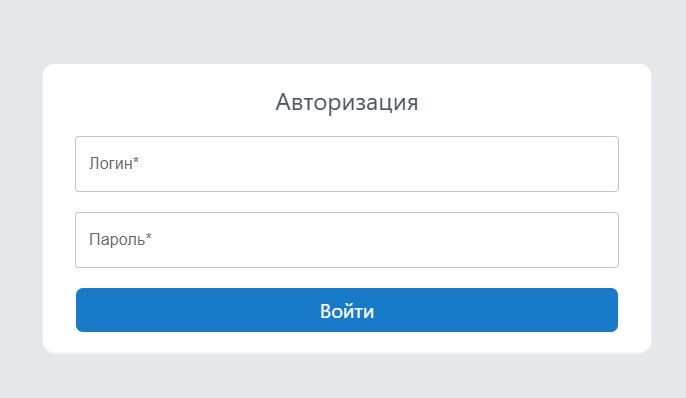
\includegraphics[scale = 0.8]{img/pages/page-01.jpg}}
		\caption{Страница авторизации}
		\label{fig:page-01}
	\end{center}
\end{figure}

\begin{figure}[H]
	\begin{center}
		{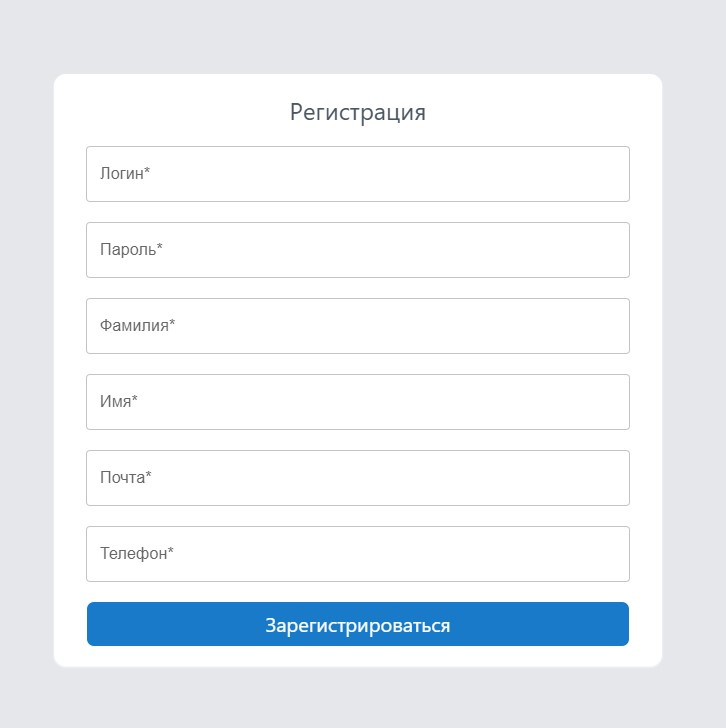
\includegraphics[scale = 0.7]{img/pages/page-02.jpg}}
		\caption{Страница регистрации}
		\label{fig:page-02}
	\end{center}
\end{figure}

\begin{figure}[H]
	\begin{center}
		{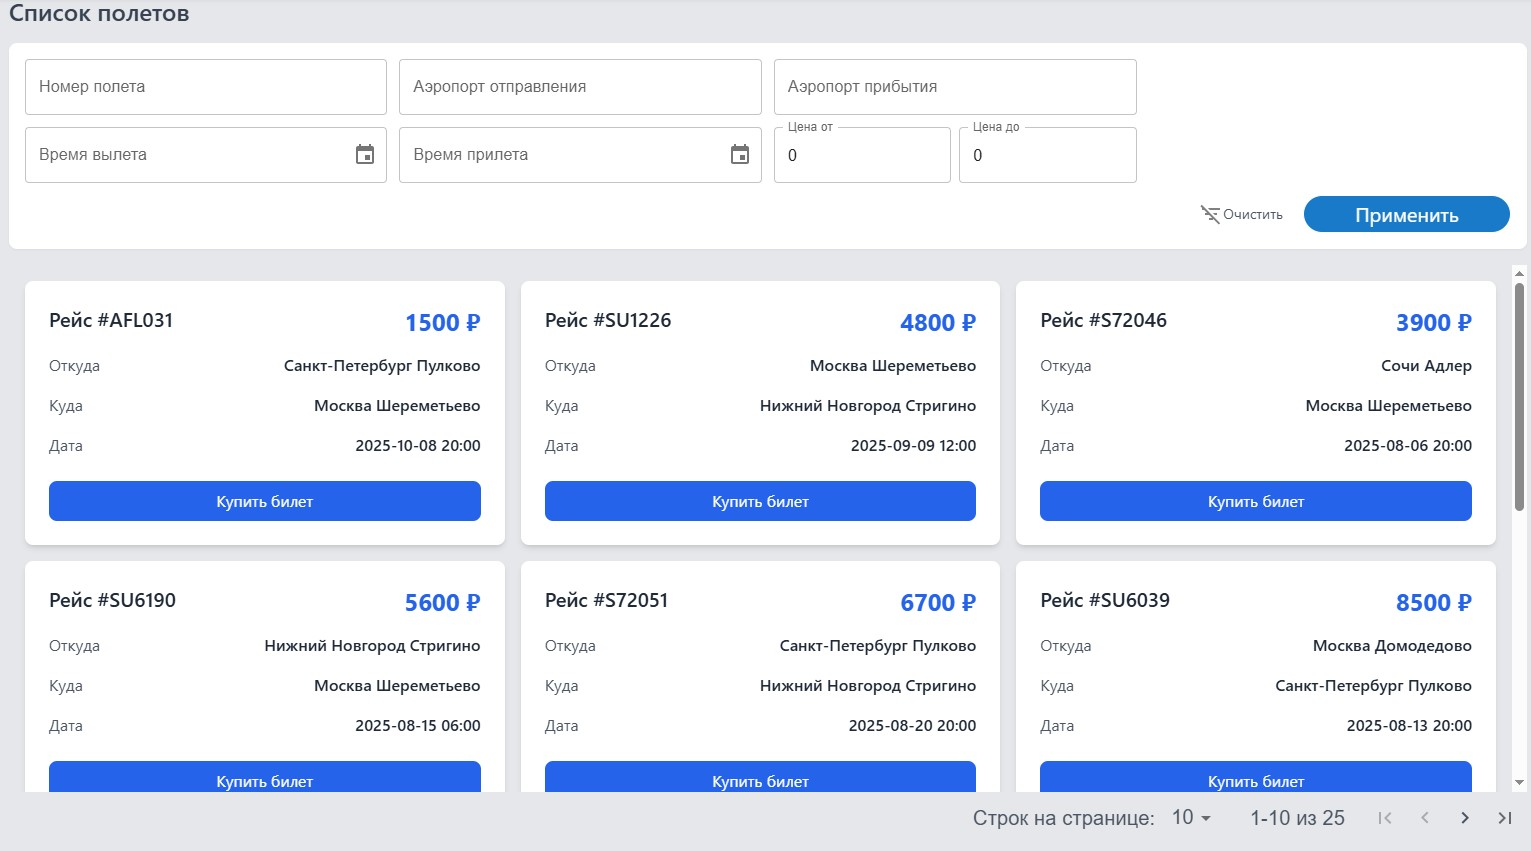
\includegraphics[scale = 0.35]{img/pages/page-03.jpg}}
		\caption{Страница с полетами (пример сортировки и фильтрации)}
		\label{fig:page-03}
	\end{center}
\end{figure}

\begin{figure}[H]
	\begin{center}
		{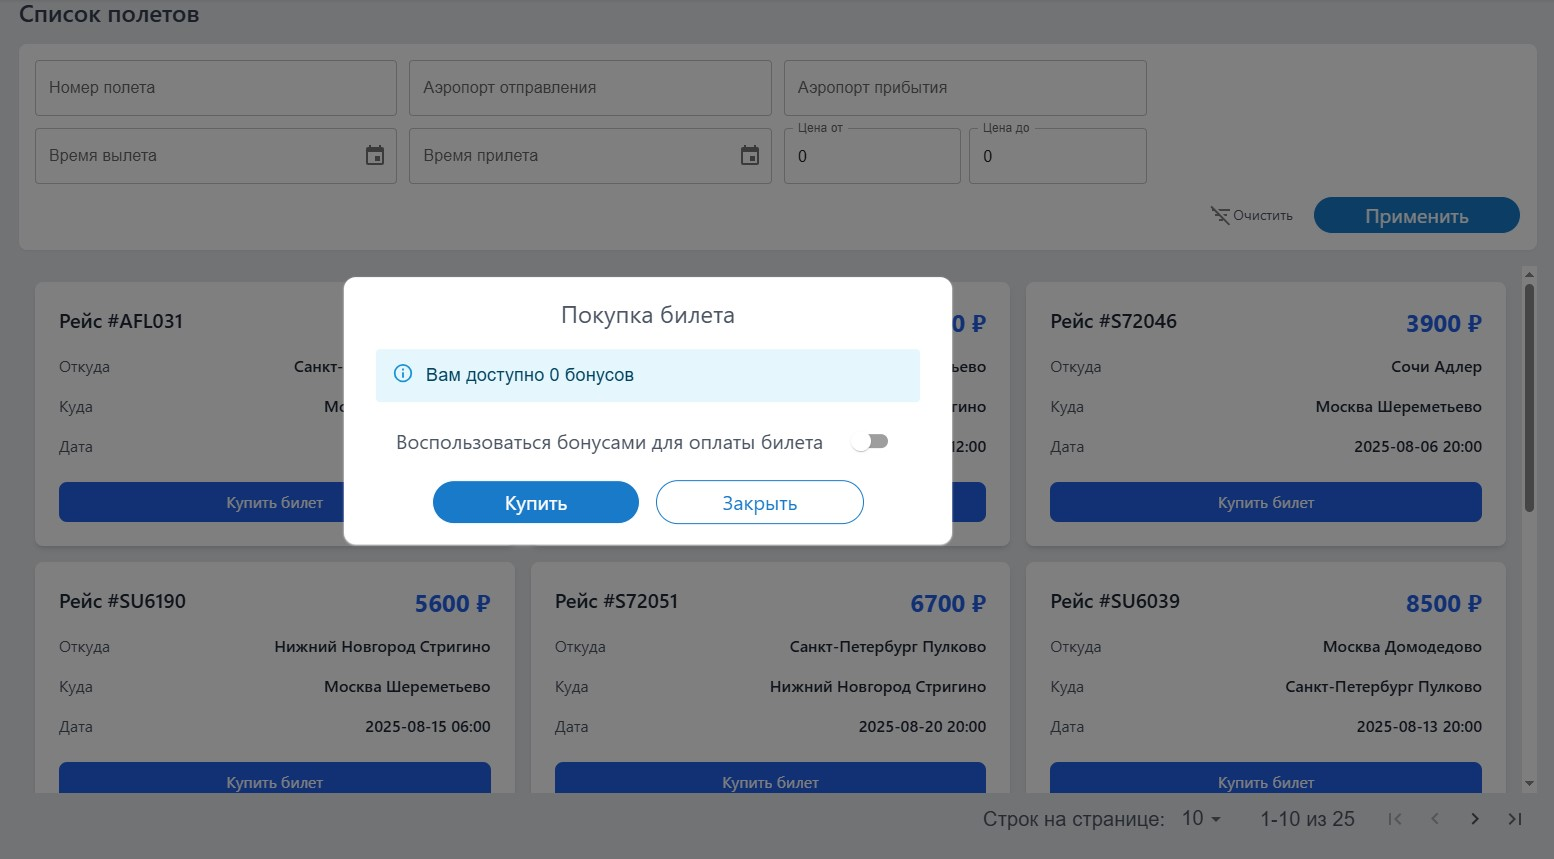
\includegraphics[scale = 0.35]{img/pages/page-04.jpg}}
		\caption{Страница с полетами (пример покупки билета)}
		\label{fig:page-04}
	\end{center}
\end{figure}

\begin{figure}[H]
	\begin{center}
		{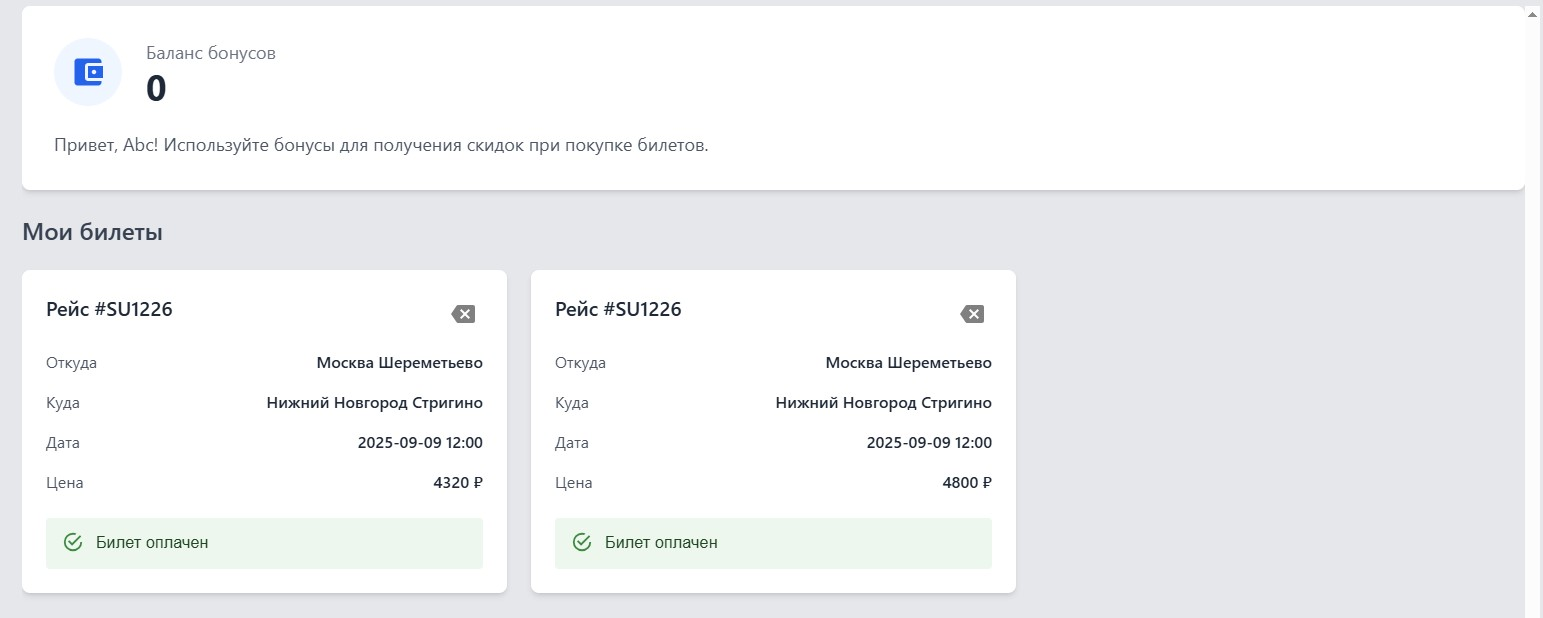
\includegraphics[scale = 0.4]{img/pages/page-05.jpg}}
		\caption{Страница с купленными и сданными билетами}
		\label{fig:page-05}
	\end{center}
\end{figure}

\begin{figure}[H]
	\begin{center}
		{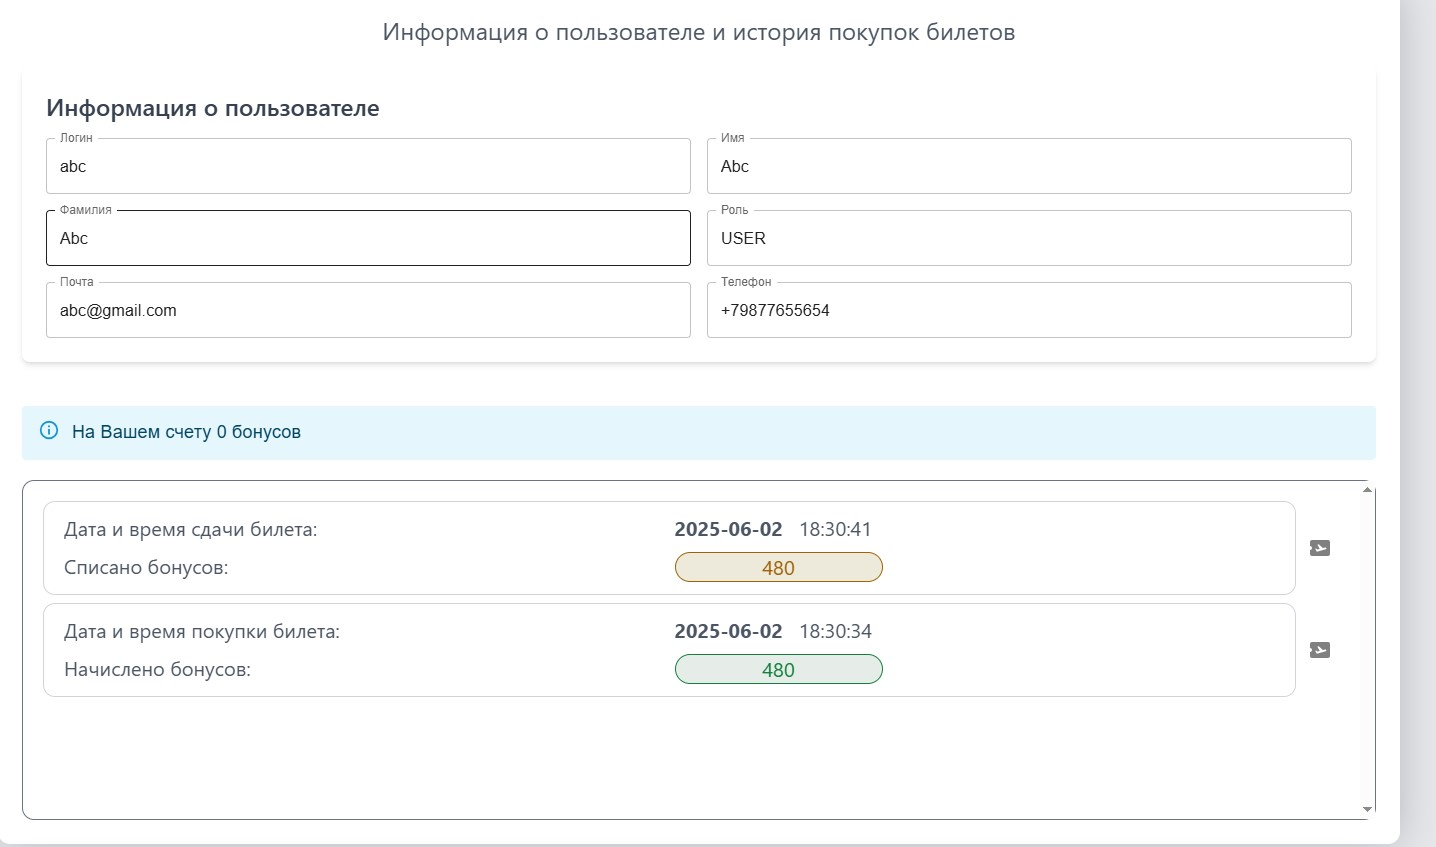
\includegraphics[scale = 0.4]{img/pages/page-06.jpg}}
		\caption{Страница с информацией о пользователе и историей покупок}
		\label{fig:page-06}
	\end{center}
\end{figure}

\begin{figure}[H]
	\begin{center}
		{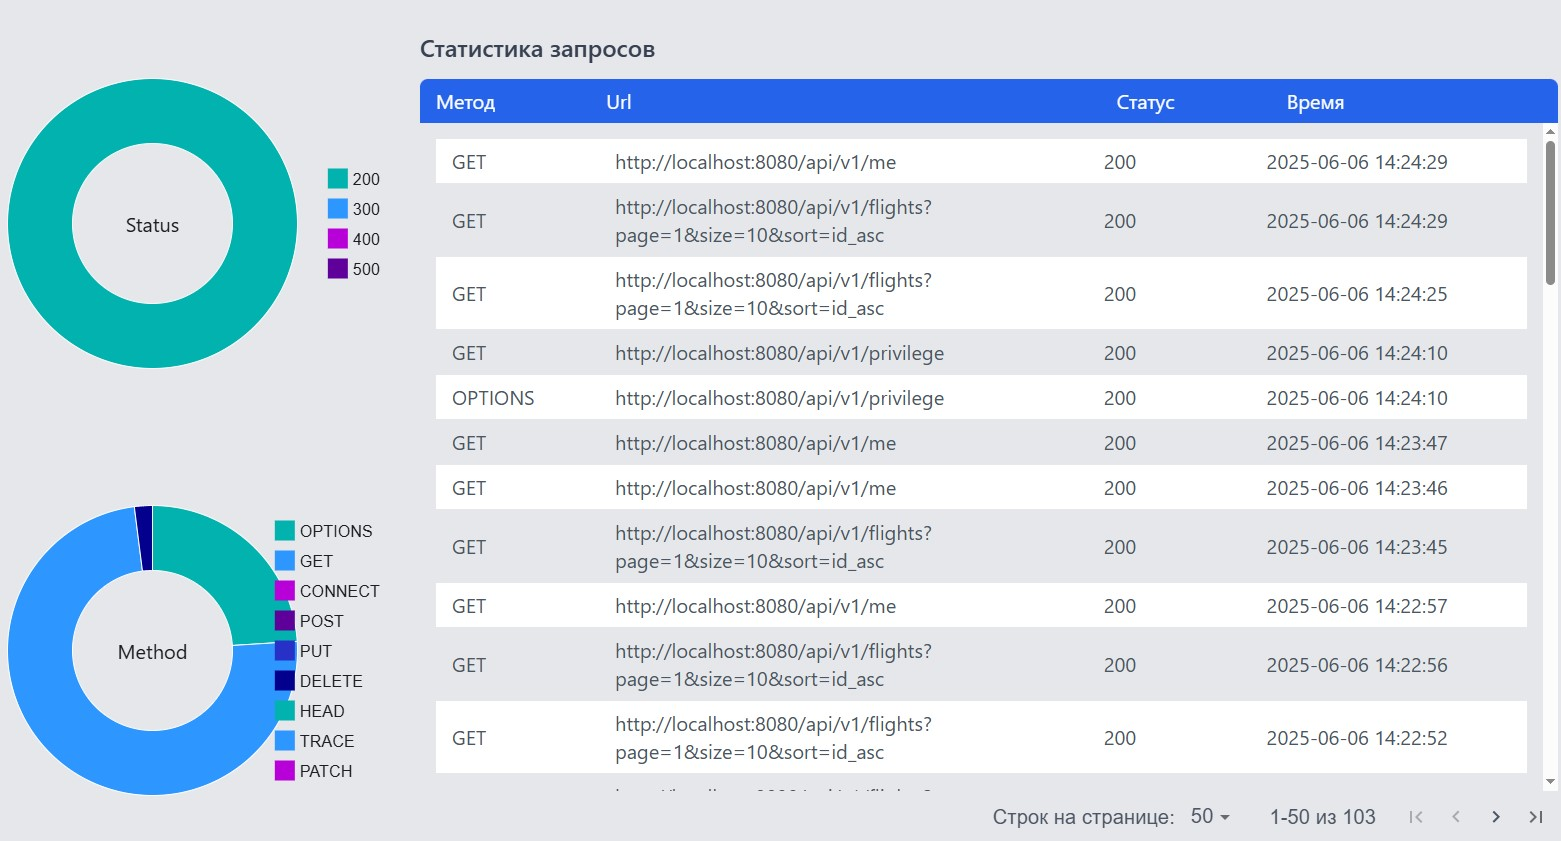
\includegraphics[scale = 0.4]{img/pages/page-07.jpg}}
		\caption{Страница со статистикой}
		\label{fig:page-07}
	\end{center}
\end{figure}

	% \chapter{Сравнение методов обнаружения глубокой подделки в изображениях}

Ниже, на таблицы \ref{analis}, показан сранительный анализ существующих методов обнаружения глубокой подделки в изображениях.

\begin{table}[H]
    \centering
    \caption{Сранительный анализ существующих методов обнаружения глубокой подделки в изображениях}\label{analis}
    \begin{NiceTabular}{*{1}{m{7em}}*{1}{C{5em}}*{2}{C{7em}}}[hvlines]
		\hline
        \centering \textit{Метод} & \textit{Высокая точность} & \textit{Автоматизация} & \textit{Зависит от изображения}\\ 
	Метод быстрого преобразования Фурье &  -- &  -- &  + \\ 
  
        Метод анализа качества изображения &  -- &  + &  + \\
        
        Нейронные сети &  + &   + & -- \\ 
        
    \end{NiceTabular}   
\end{table}

Метод быстрого преобразования Фурье подходит для частотного анализа и обнаружения аномалий, но не эффективно при обработке сложных и разнообразных данных изображений, как в случае с глубокой подделкой. На точность метода быстрого преобразования Фурье влияют условия освещения и качество входного изображения. Если изображение имеет много шума или плохую детализацию, результаты анализа могут быть неточными.

Метод анализа качества изображения (IQM) предоставляет метод оценки качества изображения, но может быть недостаточно мощным для обнаружения глубокой подделки, созданной с помощью сложных методов. Некоторые показатели IQM могут быть недостаточно чувствительными, чтобы различать изменения, возникающие в результате естественного редактирования, и изменения, возникающие в результате создания глубокой подделки. Качество и разрешение исходного изображения могут повлиять на результаты метода. Изображения низкого качества или с большим количеством шума могут привести к неточным результатам оценки.

Нейронные сети отличаются высокой степенью автоматизации и очень высокой точностью, что делает их лучшим выбором в современной технологии распознавания глубокой подделки. Нейронные сети способны анализировать и обучаться на больших объемах данных изображений, что позволяет им обнаруживать глубокую подделку с высокой точностью. Кроме того, нейронные сети можно использовать для обнаружения множества различных типов глубокой подделки.

\chapter{Постановка задачи}

Ниже, на рисунке \ref{idef}, представлена IDEF0-диаграмма нулевого уровня.

\captionsetup{justification=centering,singlelinecheck=off}
\begin{figure}[h!]
	\centering
		\includegraphics[,scale=0.75]{./img/idef0.png}
		\caption{IDEF0-диаграмма нулевого уровня}  
		\label{idef}
\end{figure}

Метод выявления обнаружения глубокой подделки в изображениях использует сверточную нейронную сеть. После построения модели сверточной нейронной сети с использованием набора данных модель определит, являются ли входные изображения поддельными или нет.
	%\setupsectionstar
\part*{ЗАКЛЮЧЕНИЕ}
\addcontentsline{toc}{part}{ЗАКЛЮЧЕНИЕ}
В рамках данной курсовой работы была разработана система для бронирования авиабилетов. В качестве фреймворка для бэкенда использовался FastAPI, для фронтенда был выбран React. В ходе выполнения работы была решена задача интеграции бэкенда и фронтенда через REST API, что обеспечило взаимодействие между клиентом и сервером. Для сбора статистики результатов запросов к сервису-координатору был использован брокер сообщений Kafka. Также была реализована авторизация и аутентификации пользователей с использованием JWT (JSON Web Token), что обеспечило защиту данных и доступ к сервису только авторизованным пользователям.

Таким образом, были решены следующие задачи, а цель достигнута.
\begin{itemize}[label = ---]
  \item Описана разрабатываемая система.
  \item Сформулированы требования к системе бронирования авиабилетов.
  \item Спроектирована архитектура распределенной системы.
  \item Произведен выбор стека технологий для реализации системы.
  \item Реализована распределенная система бронирования авиабилитов.
\end{itemize}


    \printbibliography[title=\centerline{СПИСОК ИСПОЛЬЗОВАННЫХ ИСТОЧНИКОВ}]
	\addcontentsline{toc}{part}{\textbf{СПИСОК ИСПОЛЬЗОВАННЫХ ИСТОЧНИКОВ}}
	% \begin{center}
\begin{lstlisting}[caption = Грамматика языка Oberon]
grammar oberon;

ident: IDENT;
qualident: ident;
identdef: ident '*'?;

integer: (DIGIT+);
real: DIGIT+ '.' DIGIT* ;
number: integer | real;

constDeclaration: identdef '=' constExpression;
constExpression: expression;

typeDeclaration: identdef '=' type_;
type_ : qualident | arrayType;
arrayType: ARRAY length OF type_;

length: constExpression;

identList: identdef (',' identdef)*;
variableDeclaration: identList ':' type_;

expression: simpleExpression (relation simpleExpression)?;
relation: '=' | '#'| '<'| '<='| '>'| '>=';
simpleExpression: ('+' | '-')? term (addOperator term)*;
addOperator: '+'| '-'| OR;
term: factor (mulOperator factor)*;
mulOperator: '*'| '/'| DIV| MOD| '&';

factor: number| STRING| designator (actualParameters)?| '(' expression ')'| '~' factor;
designator: qualident selector*;
selector: '[' expList ']';
expList: expression (',' expression)*;
actualParameters: '(' expList? ')';
statement: (assignment| ifStatement| whileStatement| forStatement)?;
assignment: designator ':=' expression;
statementSequence: statement (';' statement)*;
ifStatement: IF expression THEN statementSequence (ELSIF expression THEN statementSequence)* (ELSE statementSequence)? END;
whileStatement: WHILE expression DO statementSequence (ELSIF expression DO statementSequence)* END;
forStatement: FOR ident ':=' expression TO expression (BY constExpression)? DO statementSequence END;
declarationSequence: (CONST (constDeclaration ';')*)? (TYPE (typeDeclaration ';')*)? (VAR (variableDeclaration ';')*)?;

module: MODULE ident ';' declarationSequence (BEGIN statementSequence)? RETURN factor ';' END ident '.' EOF;

ARRAY: 'ARRAY';
OF: 'OF';
END: 'END';
TO: 'TO';
OR: 'OR';
DIV: 'DIV';
MOD: 'MOD';
IF: 'IF';
THEN: 'THEN';
ELSIF: 'ELSIF';
ELSE: 'ELSE';
WHILE: 'WHILE';
DO: 'DO';
FOR: 'FOR';
BY: 'BY';
BEGIN: 'BEGIN';
RETURN: 'RETURN';
TYPE: 'TYPE';
VAR: 'VAR';
MODULE: 'MODULE';
STRING: ('"' .*? '"')| (DIGIT HEXDIGIT* 'X');
IDENT: LETTER (LETTER | DIGIT)*;
LETTER: [a-zA-Z];
DIGIT: [0-9];
COMMENT: '(*' .*? '*)' -> skip;
WS: [ \t\r\n] -> skip;
\end{lstlisting}
\end{center}

\pagebreak
\end{document}